\chapter{Grafičko sučelje}

Aplikacija za testiranje realizirana je kao \textit{desktop} aplikacija,
korištenjem Qt i Qt3D biblioteka. Glavni prozor aplikacije sastoji se od 
3D prikaza u kojem je moguće vidjeti modele koji su trenutno učitani, a
u donjem dijelu glavnog prozora vidljiv je prozor informacija \textit{log box}
u kojem je moguće vidjeti izmjerene performanse. (Slika \ref{gui})

Aplikacija se pokreće tako da se izvršna datoteka pozove s 2 argumenta koji moraju
biti putanje do dviju \textit{.obj} datoteka. Moguće je proslijediti i dodatni argument
(\textit{--bruteforce}), kojim će se pokrenuti i testiranje metodom grube sile.

\begin{figure}[h!]
    \centering
    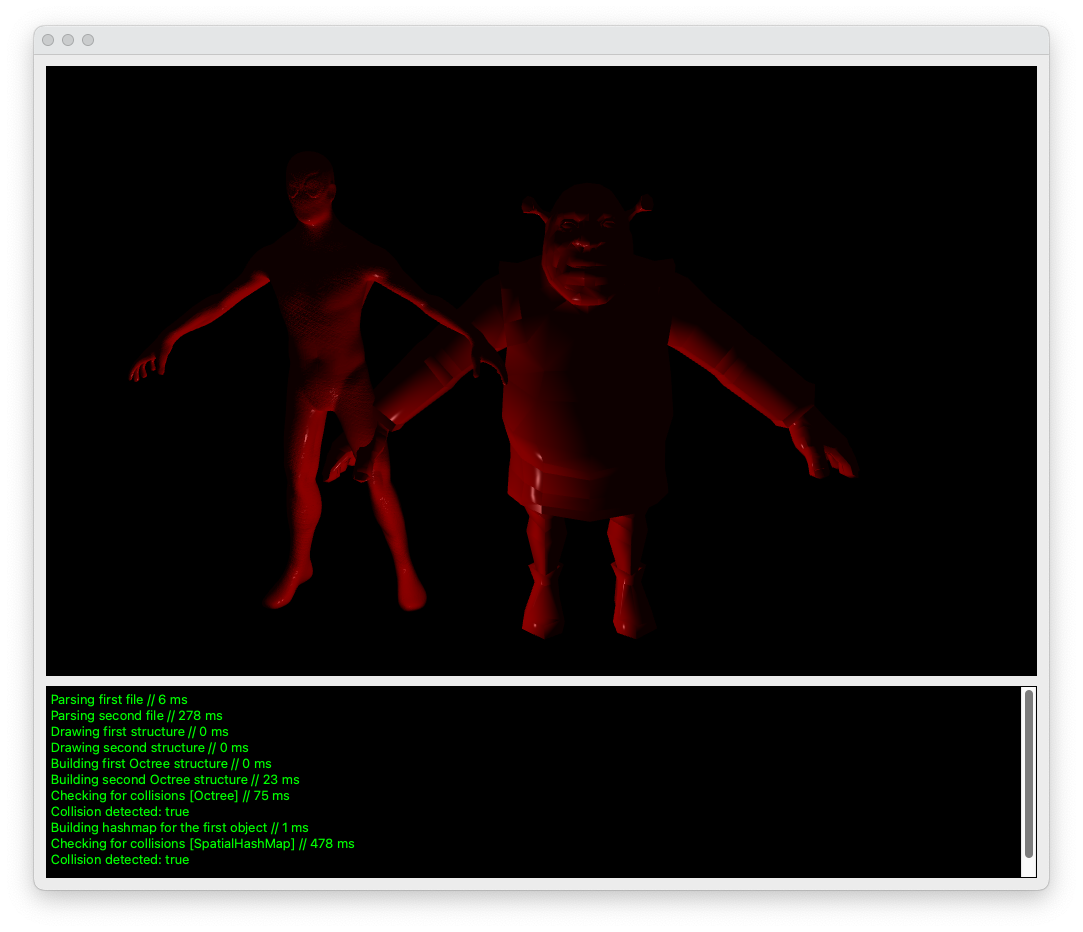
\includegraphics[width=12cm]{gui.png}
    \caption {Izgled glavnog prozora aplikacije}
    \label{gui}
\end{figure}

Trajanje svakog koraka algoritma izmjereno je korištenjem \textit{chrono} biblioteke.
Nakon što se algoritam izvrši, modele je moguće vidjeti u glavnom prozoru, a rezultate
testiranja u donjem prozoru za informacije.

\begin{cppSource}{Implementacija funkcije za grafički prikaz modela}
void View3D::add_obj_file(std::string filename) {
    Qt3DCore::QEntity *mesh_entity = new Qt3DCore::QEntity(this->root_entity);
    Qt3DRender::QMesh *mesh = new Qt3DRender::QMesh(this->root_entity);
    mesh->setSource(QUrl::fromLocalFile(filename.c_str()));

    mesh_entity->addComponent(mesh);
    mesh_entity->addComponent(this->phong_red);
}
\end{cppSource}

\begin{cppSource}{Dio koda za mjerenje trajanja funkcije}
...
start_time = chrono::high_resolution_clock::now();
*(log_box) << "Checking for collisions [Octree] // ";
bool octree_collides = tree1.collides(&tree2);
int duration = chrono::duration_cast<chrono::milliseconds>(
    chrono::high_resolution_clock::now() - start_time
).count();
*(log_box) << duration << " ms\n";
*(log_box) << "Collision detected: "
           << (octree_collides ? "true" : "false") << "\n";
...
\end{cppSource}
